\chapter{Hardware}
\label{cha:hardware}

Największą częścią projektu było wykonanie hardware'u słuchawek. Dobór parametrów elementów akustycznych był szczególnie trudny, biorąc pod uwagę brak doświadczenia w tym obszarze elektroniki. Wszystkie elementy schematu musiały być wybrane pod kątem minimalizacji szumów i poboru mocy, a zaprojektowana płytka musiała się zmieścić do obudowy słuchawek i pozwolić na wyprowadzenie na zewnątrz mikrofonu, przycisków oraz gniazda ładowania. To wymagało przemyślanego wymiarowania zarówno modelu, jak i płytki oraz wyprowadzenia w odpowiedni sposób elementów, na przykład stosując kątowe przyciski.

Dla projektu obudowy głównym ograniczeniem było to, aby słuchawki były kompaktowe, czyli lekkie i niskoprofilowe. Ochronniki tego typu są przeznaczone dla myśliwych, strzelców sportowych, ale również dla służb ochrony i wojsk specjalnych. Toteż nie mogą ograniczać ruchów, możliwości przyłożenia głowy do kolby broni i być znaczącym ciężarem podczas użytkowania przez kilka godzin lub dni w terenie.

Ten sam powód determinuje wymóg niskiego poboru prądu przez układ i dużej pojemności akumulatora. Choć w tej pracy został wybrany wbudowany akumulator ładowany przez gniazdo mikro USB, to do zastosowań wojskowych lepsze byłoby zasilanie ze zwykłych, wymiennych baterii, na przykład AAA.

Układy scalone zastosowane w projekcie musiały mieć możliwość zasilania napięciem 3.3V, ponieważ zastosowany został akumulator litowo-jonowy o napięciu znamionowym $3,7V$ (zakres pracy wynosi od $3,0$ do $4,2V$).

Dla uproszczenia, podczas wyboru komponentów nie była brana pod uwagę wodo- oraz kurzoodporność i zakres temperatur pracy. Jednak gdyby słuchawki miały wejść na rynek, musiałyby zostać dodatkowo przystosowane do działania w wymagających warunkach terenowych.


\section{Układ elektroniczny}
\label{cha:uklad}

Przed przystąpieniem do projektowania właściwego układu elektronicznego konieczne było zadecydowanie, czy wykonać go analogowo, czy cyfrowo. Podejście pierwsze oznaczało użycie inwerterów, wzmacniaczy, filtrów, itp. do uzyskania odpowiednich opóźnienia i fazy dźwięku. Jednak pozostawała wciąż kwestia możliwości zamiennego wyciszania i przekazywania dźwięków w zależności od ich amplitudy. Okazało się, że znalezienie materiałów na ten temat jest wyjątkowo trudne, a szukanie błędów na schemacie mogłoby sprawiać dużo więcej problemów, niż w programie na mikrokontroler. Z tego powodu został wybrany układ cyfrowy, który jak się później okazało, powodował wiele problemów z szumami i opóźnieniami sygnału.

Kolejną decyzją do podjęcia było to, czy każda ze słuchawek będzie miała swój własny układ, czy też jedna będzie odpowiedzialna za obliczenia, a druga jedynie skomunikowana z nią. Zostało wybrane podejście drugie, ponieważ pozwalało to zminimalizować koszty oraz lepiej rozłożyć masę. Jedna słuchawka miała zawierać główną płytkę z mikrokontrolerem i przyciskami, a druga jedynie mikrofon oraz układ ładowania i akumulator. Wadą tego rozwiązania była konieczność równoczesnej analizy dźwięków z obu słuchawek, co przekładało się na szybkość działania mikrokontrolera oraz narażone na szumy przewody prowadzące przez pałąk od jednej słuchawki do drugiej.

Poniżej przedstawiono uproszczony schemat układów dla obu słuchawek.

\textbf{SCHEMAT UKŁADÓW SŁUCHAWEK}


\section{Głośniki}
\label{cha:glosniki}

Każda ze słuchawek została wyposażona w głośnik odpowiedzialny zarówno za doprowadzanie do ucha zwykłych dźwięków z zewnątrz, jak i generowanie antyfazy dla dźwięków niebezpiecznych. Wybrany został głośnik \textit{254-PS604-RO} firmy \textit{Kobitone}. Głównym kryterium wyboru była impedancja głośnika, wynosząca $32\Omega$ oraz moc znamionowa na poziomie $ 200 mW $. Te parametry zapewniały dobrą jakość odtwarzanego dźwięku, która była kluczowa, aby uzyskać maksymalne odwzorowanie dźwięków otoczenia. Celem było to, aby użytkownik czuł się w słuchawkach naturalnie. Choć charakterystyka częstotliwościowa głośnika jest zbliżona do liniowej tylko w zakresie od $ 400 $ do $ 7000 Hz $, to zawiera się w nim większość słyszanych odbieranych przez człowieka dźwięków.

Sterowanie głośnikami zostało przewidziane z wykorzystaniem wbudowanych w mikrokontroler dwóch 12-bitowych przetworników cyfrowo-analogowych w trybie single-ended. Ich wyjścia były dodatkowo wzmacniane przez układy \textit{TPA2005D1DGNR} firmy \textit{Texas Instruments}. Są to wzmacniacze audio klasy D, stworzonej na potrzeby urządzeń przenośnych. Obok innych popularnych klas, jak A, B, AB, czy G, klasa D charakteryzuje się bardzo wysoką wydajnością mocową (nawet powyżej $ 90\% $). Wynika ona stąd, że w odróżnieniu od pozostałych, gdzie stosowane są konfiguracje common-emitter lub push-pull, klasa D stosuje całkowite załączanie lub wyłączanie tranzystora wyjściowego i modulację częstotliwości PWM, aby przybliżyć analogowy poziom napięcia\cite{AudioAmps}. Układ \textit{TPA2005D1} ma według specyfikacji wydajność ok. $ 85\% $ przy $32\Omega$ głośniku, zasilaniu $ 3.6V $ i mocy wyjściowej $ 100mW $.

Dodatkowo układy te mają wbudowany pin shutdown, który został użyty aby wyłączać je w trybie uśpienia słuchawek opisanym szerzej w rozdziale \ref{cha:soft_sys}. Dzięki niemu wzmacniacze mogą pobierać zaledwie $ 0.5 µA $.

W idealnym przypadku słuchawki powinny zawierać kilka głośników, co umożliwiłoby symulację dźwięku przestrzennego. To jednak zwiększyłoby koszt słuchawek, wymagało zamontowania kilku mikrofonów, utrudniło rozmieszczenie elementów wewnątrz i implementację algorytmu wyciszającego.


\section{Mikrofony}
\label{cha:mikrofony}

Wybór mikrofonu był największym problemem ze względu na różne technologie wykonania (elektretowy, MEMS) oraz dużo parametrów. Początkowo miał zostać użyty mikrofon elektretowy, jednak okazało się, że są one mało precyzyjne. Konieczne było wybranie technologii MEMS, czyli miniaturowego mikrofonu wbudowanego w chip z otworem do akwizycji fal akustycznych.

\begin{figure}[H]
	\centering
	\begin{subfigure}{.45\textwidth}
		\centering
		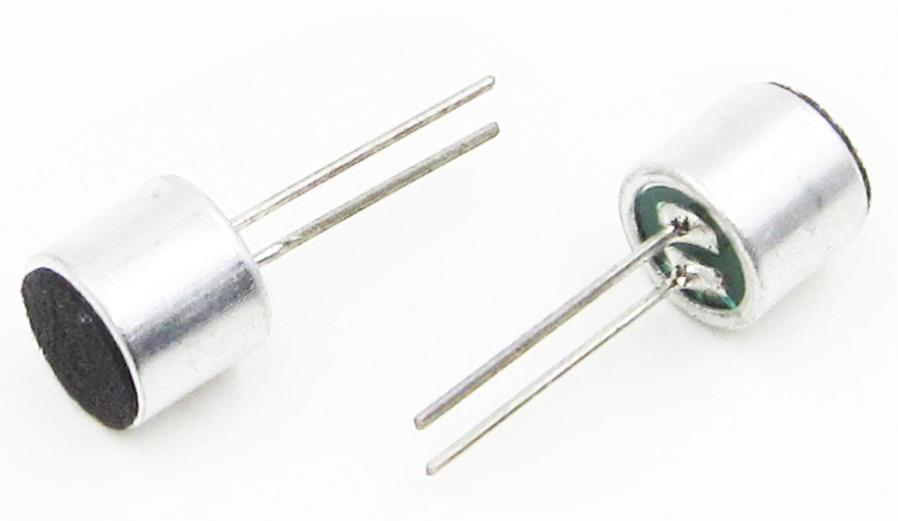
\includegraphics[height=3.5cm]{zdjecia/mic_electret.jpg}
		\subcaption{Mikrofon eletretowy}
	\end{subfigure}
	\begin{subfigure}{.45\textwidth}
		\centering
		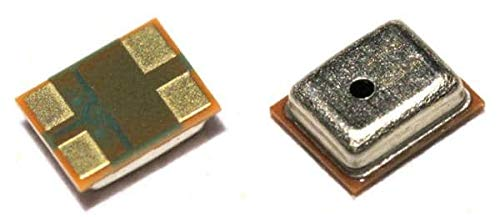
\includegraphics[height=3.5cm]{zdjecia/mic_mems.jpg}
		\subcaption{Mikrofon MEMS}
	\end{subfigure}
	\caption{\label{mikrofony} Mikrofony w różnych technologiach}
\end{figure}

Do celów projektu wybrany został mikrofon \textit{SPW2430HR5H-B} firmy \textit{Knowles}. Ponieważ jest to urządzenie on-chip, konieczne było dostosowanie projektu tak, aby płytka była maksymalnie blisko zewnętrznej ścianki obudowy. Port do akwizycji znajduje się w górnej części elementu i jest odsunięty o $ 1mm $ od dolnej części, a więc ok. $ 1mm $ od powierzchni PCB.
Jednym z głównych kryteriów wyboru była czułość. Informuje ona, jaka amplituda sygnału wyjściowego mikrofonu odpowiada danemu poziomowi ciśnienia akustycznego. W specyfikacji podawana jest jako ujemna wartość $dBV/Pa$ mierzona falą akustyczną o częstotliwości $1kHz$ i SPL $94dB$. Jednostka $dBV$ oznacza liczbę decybeli w odniesieniu do $1V$\cite{MicSens}. Stąd wzór na czułość wygląda następująco:

\begin{equation}
Sensitivity_{dBV} = 20 \cdot log_{10}\frac{Sensitivity_{mV/Pa}}{Output_{REF}}
\end{equation}

gdzie: \\
\indent$Sensitivity_{dBV}$ - czułość w dBV/Pa \\
\indent$Sensitivity_{mV/Pa}$ - czułość w mV/Pa \\
\indent$Output_{REF}$ - wyjściowe napięcie odniesienia ($1000mV/Pa$) 

Powyższy wzór można przekształcić, aby z podanej w nocie katalogowej czułości obliczyć poziom napięcia dla danego SPL.
\begin{equation}
Sensitivity_{mV/Pa} = 1000 \cdot 10^{\frac{Sensitivity_{dBV}}{20}}
\end{equation}

Wybrany mikrofon ma średnią czułość $-42 dbV/Pa$, a więc zgodnie ze wzorem $7,943 mV/Pa$. Stąd przy poziomie ciśnienia akustycznego $1Pa$ zmiana sygnału wyjściowego mikrofonu wyniesie $7,943 mV$. Według specyfikacji maksymalny poziom SPL to $129 dB$, czyli $56,37 Pa$. Maksymalną zmianą napięcia wyjściowego mikrofonu powinno być więc $447,75 mV$.

Czułość mikrofonu jest zwykle odwrotnie proporcjonalna do jego maksymalnego SPL. Dlatego w projekcie słuchawek strzeleckich, które są przeznaczone do nasłuchiwania zarówno skrajnie cichych, jak i skrajnie głośnych dźwięków, zastosowanie jednego mikrofonu wymaga kompromisu między oboma parametrami. 

Rozwiązaniami w tej sytuacji byłoby zastosowanie dwóch mikrofonów o różnych czułościach lub dodanie wzmacniacza sterowanego przez oprogramowanie. Pierwsze z nich gwarantuje dobrą akwizycję wszystkich poziomów dźwięków, jednak jest wyzwaniem pod względem konstrukcyjnym, wymaga użycia większej liczby przetworników analogowo-cyfrowych i sprawnego przełączania przetwarzania przez oprogramowanie. Drugie zaś bazowałoby na mikrofonie o małej czułości i przy małych natężeniach dźwięku zwiększaniu jego amplitudy wyjściowej przez wzmacniacz sterowany potencjometrem cyfrowym. To rozwiązanie wydaje się być lepsze, choć również wymaga zaprogramowania portów mikrokontrolera tak, aby dostosowywały wzmocnienie.

W tym konkretnym przypadku problemem jest konieczność przetwarzania dźwięków o amplitudach przekraczających $140dB$
\textbf{REFERENCJA}
Znalezienie mikrofonu z takim wysokim progiem jest bardzo trudne, dlatego prawdopodobnie konieczne by było mechaniczne wyciszenie dźwięków docierających do mikrofonu, aby obniżyć odbierany poziom ciśnienia akustycznego.

Słuchawki zostały dodatkowo zaprojektowane tak, aby była możliwość podłączenia ich do radiotelefonu. Do tego celu został wybrany jeszcze jeden mikrofon montowany w elastycznej rurce przed ustami użytkownika i umożliwiający rozmowę z użyciem komunikacji radiowej. W tym przypadku jest to mikrofon elektretowy \textit{CMEJ-4622-25-L082}, ponieważ jego montaż nie wymaga padów lutowniczych. Nie było konieczne wybieranie mikrofonu o dobrym SNR, ponieważ komunikacja radiowa i tak wprowadza duże szumy. Czułość mikrofonu powinna być natomiast stosunkowo mała, ponieważ odległość od źródła dźwięku jest niewielka.


\section{Mikrokontroler}
\label{cha:uC}

Jako jednostkę obliczeniową, wybrano mikrokontroler firmy \textit{STMicroelectronics}: \textit{STM32L476RG}.

Jego rdzeniem jest 32-bitowy \textit{Cortex-M4} z możliwością zastosowania bibliotek DSP (ang. \textit{Digital Signal Processing} - Cyfrowe Przetwarzanie Sygnałów). Z kolei \textit{L} jest niskoprądową alternatywą dla serii \textit{F}. Głównie tych dwóch powodów został wybrany do tych słuchawek.

Maksymalna częstotliwość zegara procesora wynosi $80MHz$. Mikrokontroler posiada 3 12-bitowe przetworniki analogowo-cyfrowe, czyli akurat tyle, aby próbkować dwa mikrofony i sygnał z radiotelefonu. Do tego 2 12-bitowe przetworniki cyfrowo-analogowe - po jednym na głośnik\cite{STM32L4}.

Na potrzeby prototypowania wykorzystano płytkę \textit{Nucleo-64}, która zawiera programator \textit{ST-LINK}, diodę oraz przycisk użytkownika, przycisk resetu i jest kompatybilna z nakładkami na popularną platformę \textit{Arduino Uno}. Miała ona zostać również użyta do zaprogramowania mikrokontrolera na docelowej płytce PCB.


\section{PCB}
\label{cha:PCB}

Projekt płytki PCB został wykonany w programie \textit{Altium Designer 6.1} na licencji AGH udostępnionej przez Promotora. Postępy były archiwizowane z użyciem systemu kontroli wersji \textit{git}. Repozytorium z projektem: \url{https://gitlab.com/Hoplophile/tactical_headphones.git}.

Zastosowano globalne etykiety połączeń i podział na pliki dla lepszej przejrzystości. Do wyglądu schematów wykorzystany został szablon stworzony w ramach zajęć \textit{Podstawy projektowania obwodów z wykorzystaniem oprogramowania CAD/CAM}. 

Ponieważ użyta wersja \textit{Altiuma} nie posiada jeszcze opcji projektu wielolayoutowego, konieczne było stworzenie dwóch podprojektów. Zostały do nich dodane odpowiednie pliki z głównego projektu. Strukturę plików przedstawiono na obrazku \ref{pic:struktura}.

\begin{figure}[H]
	\centering
	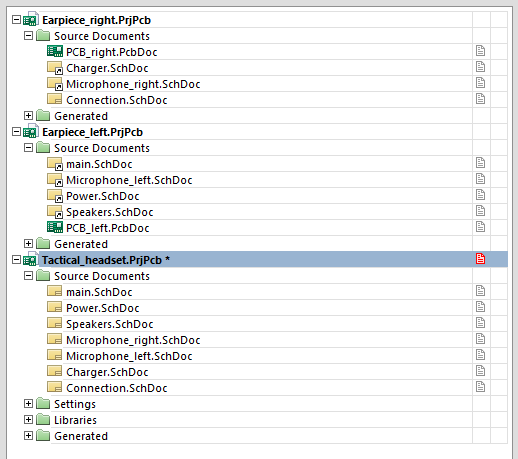
\includegraphics[scale=0.6]{zdjecia/PCB/struktura.png}
	\caption{\label{pic:struktura} Struktura plików w projektach PCB}
\end{figure}

Poniżej opisano poszczególne schematy oraz layouty składające się na projekt słuchawek.


\subsection{Main}

Plik main.sch zawiera ogólne elementy schematu, czyli: mikrokontroler, przyciski użytkownika oraz konektory do programowania, komunikacji między lewą i prawą słuchawką, mikrofonu komunikacyjnego i komunikacji radiowej.

Przewidziano 3 przyciski dla użytkownika (plus/góra, minus/dół, główny). Zostały podłączone do portów GPIO mikrokontrolera oraz do zasilania przez rezystory pull-up o wartościach $4,7k\Omega$. Wciśnięcie przycisku jest równoważne ze zwarciem danego portu do masy.

Podobnie pin \textbf{NRST} jest podłączony do zasilania przez rezystor pull-up. W pierwszych wersjach schematu był tam również podłączony przycisk TACT, jednak usunięto go, aby zaoszczędzić miejsce. Reset jest możliwy poprzez zwarcie pinu resetu na konektorze \textbf{SWD}.

Złącze do programowania jest zaprojektowane tak, aby można było flashować i debugować mikrokontroler przez złącze ST-LINK obecne na przykład na platformie Nucleo, na której wykonywany był prototyp. 

Konektor do komunikacji radiowej ma 3 piny. Pierwszy jest połączeniem do masy. Drugi przekazuje sygnał z radiotelefonu do przetwornika analogowo-cyfrowego mikrokontrolera. Trzeci jest pinem wyjściowym mikrofonu komunikacyjnego, przy którym zastosowano równolegle rezystor, ograniczający prąd zasilania mikrofonu oraz szeregowo kondensator blokujący napięcie stałe.

Do pinu $V_{REF}$ mikrokontrolera dodano dodatkowo dwa kondensatory: \textbf{C1} i \textbf{C4}. Zastosowano je później, po pierwszych próbach odczytu sygnału z mikrofonu przez wbudowany ADC, ponieważ okazało się, że jest on obarczony dużym szumem.

\begin{figure}[H]
	\centering
	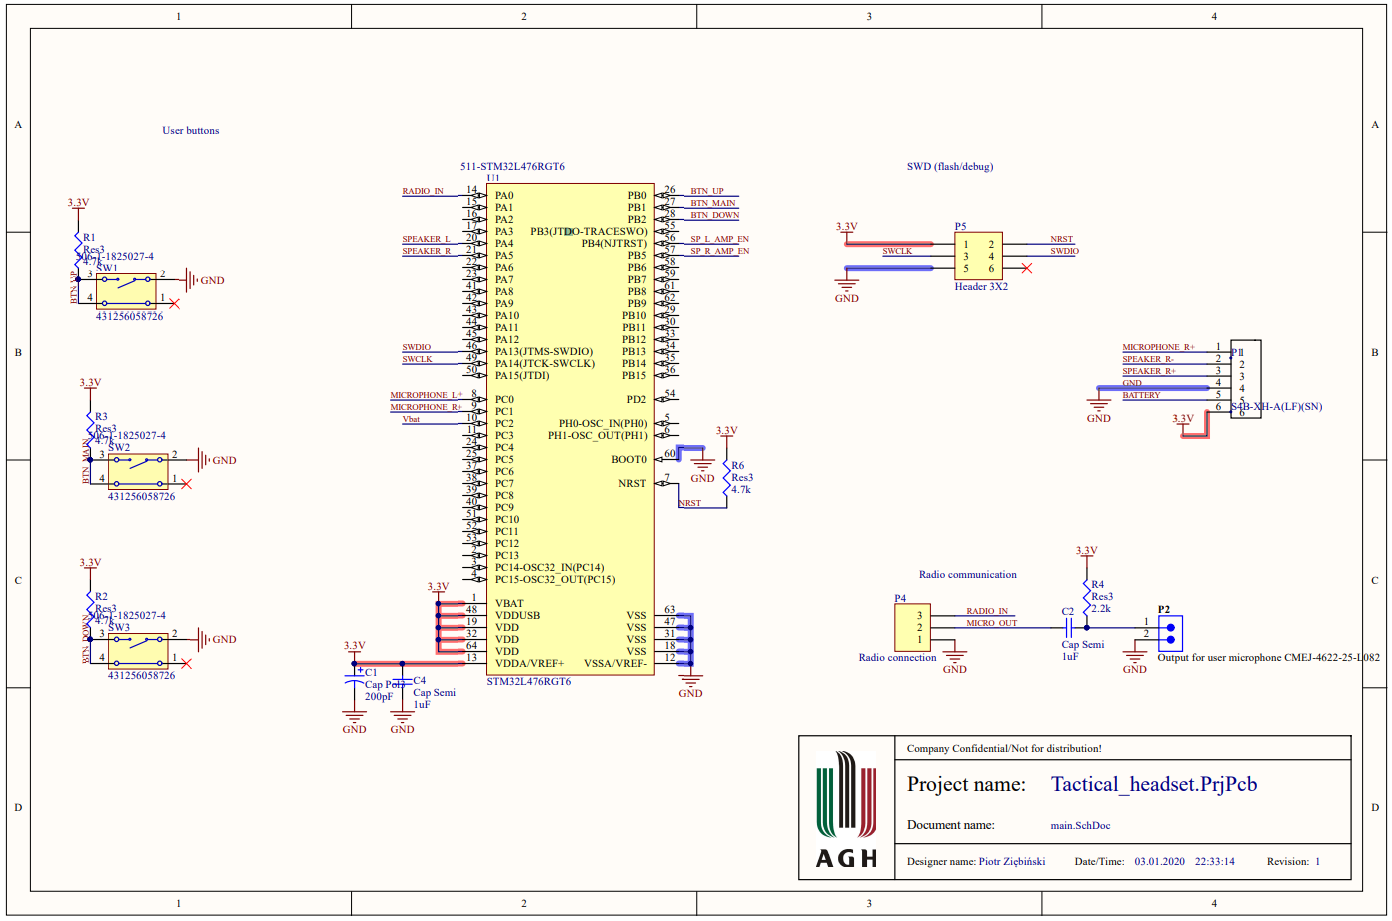
\includegraphics[scale=0.4]{zdjecia/PCB/main.png}
	\caption{\label{main} Schemat \textit{main}}
\end{figure}


\subsection{Power}

Początkowo ten plik zawierał stabilizator napięcia oraz układ ładowania do akumulatora. Na potrzeby podziału układu na dwie osobne płytki PCB, układ ładowania został przeniesiony na osobny schemat. Na głównej, lewej płytce został stabilizator \textbf{JAKI STABILIZATOR} ustawiony na $3.3V$. Według specyfikacji jest w stanie dać \textbf{PRĄD}. Zostały dodane kondensatory filtrujące oraz cewka na wyjściu, tworzące filtr dolnoprzepustowy LC o częstotliwości granicznej \textbf{CZESTOT. NA WYJŚCIU REG}. 

Miedzy portem wejściowym baterii a masą został utworzony dzielnik napięcia z rezystorami $220k \Omega $. Było to konieczne do pomiaru poziomu naładowania baterii, ponieważ jej napięcie maksymalne wynosi $4,2V$ co wykracza poza zakres przetwornika mikrokontrolera, którego $V_{ref}$ wynosi $3,3V$. Napięcie jest dzielone przez 2, więc maksymalnie wynosi $2,1V$ i mieści się w zakresie ADC, a odczytana wartość jest mnożona dwukrotnie przez program, aby otrzymać rzeczywistą wartość. Dzięki zastosowaniu rezystorów o dużej wartości, prąd przepływający przez dzielnik przy pełnym naładowaniu baterii wynosi tylko $9,6\mu A$.

\begin{figure}[H]
	\centering
	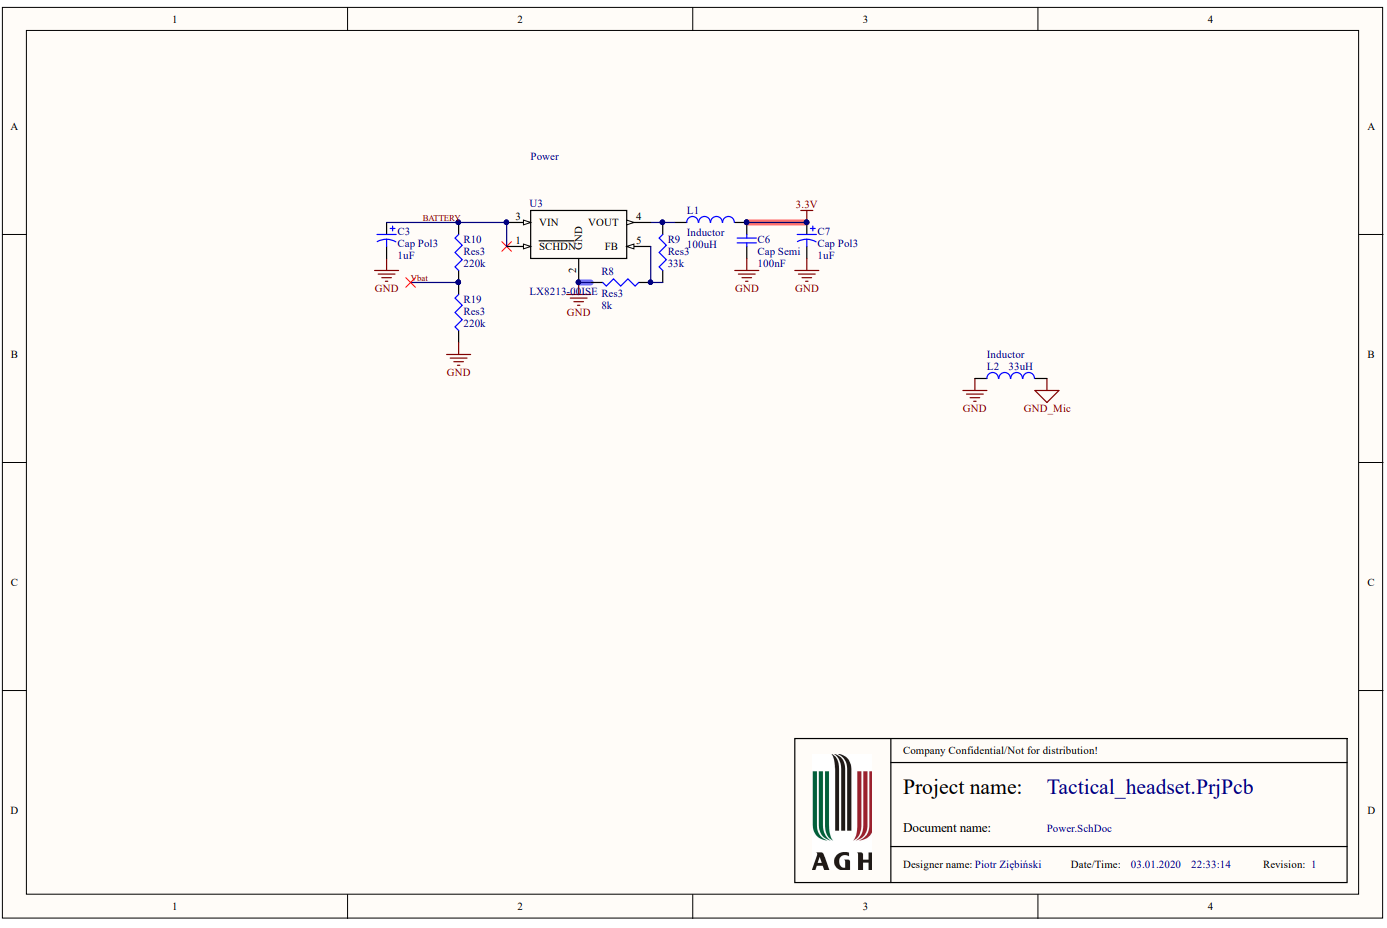
\includegraphics[scale=0.4]{zdjecia/PCB/power.png}
	\caption{\label{power} Schemat \textit{Power}}
\end{figure}


\subsection{Charger}

Układ ładujący do akumulatora został przeniesiony na osobny schemat, kiedy zdecydowano o jego umieszczeniu na drugiej płytce. Wejściem jest złącze żeńskie micro USB B, przez które dostarczane jest napięcie $5V$, natomiast wyjście jest bezpośrednio połączone z portem akumulatora. Wykorzystano również możliwość wskazywania statusu ładowania, dodając diodę LED według specyfikacji. Rezystor \textbf{R16} służy do ustawiania prądu ładowania, wybrana wartość jest równoważna z $450mA$, co jest bliskie maksymalnemu prądowi ładowania wybranego akumulatora, wynoszącemu \textbf{PRĄD ŁADOWANIA}. 

Zgodnie z zalecaną aplikacją w nocie katalogowej, dodano kondensatory na wejściu i wyjściu układu.

\begin{figure}[H]
	\centering
	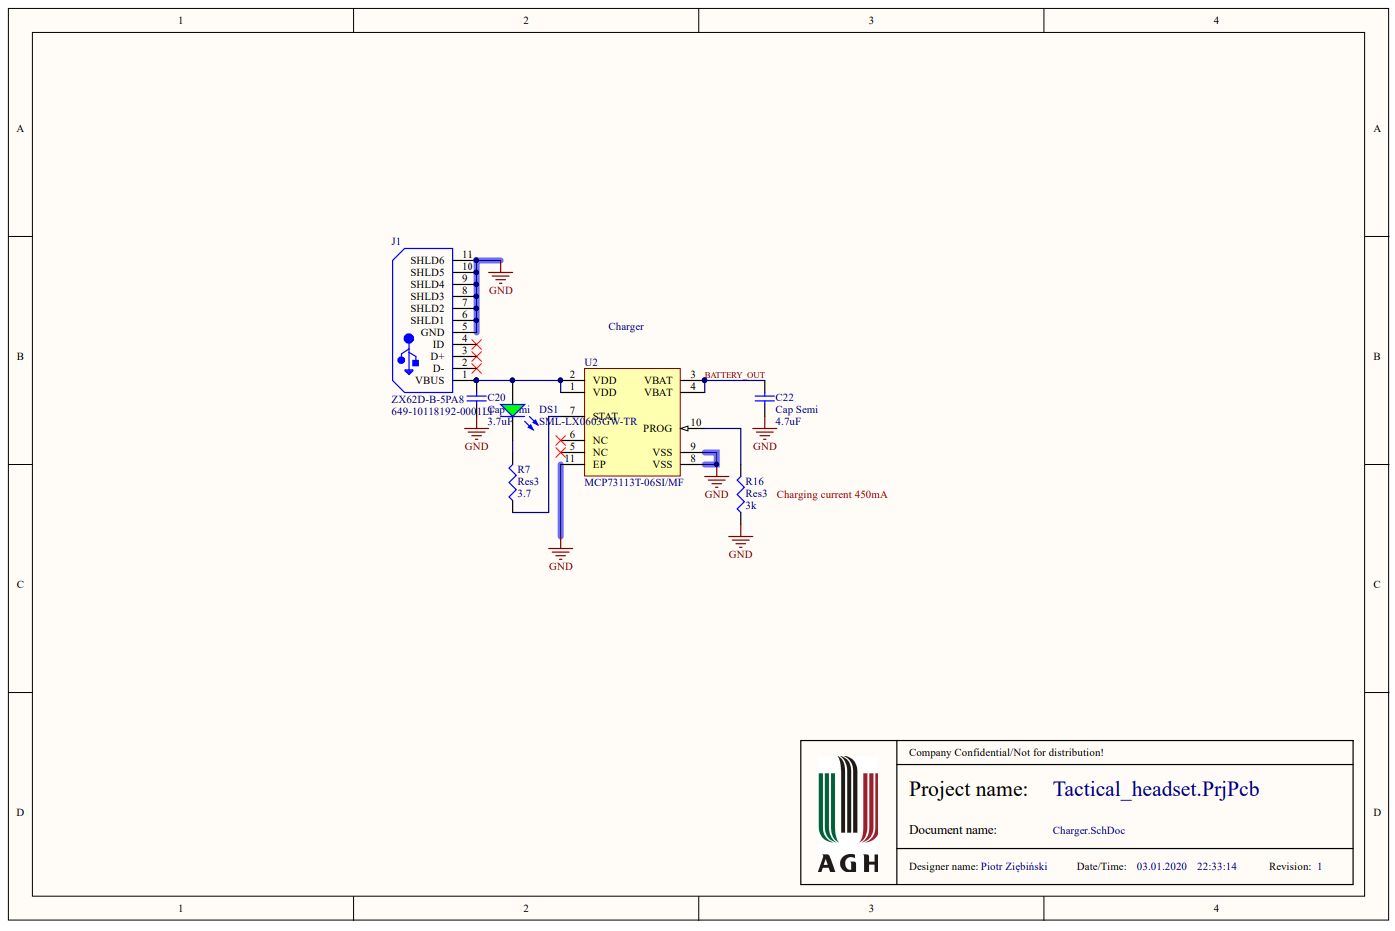
\includegraphics[scale=0.4]{zdjecia/PCB/charger.png}
	\caption{\label{charger} Schemat \textit{Charger}}
\end{figure}


\subsection{Microphone\_left i Microphone\_right}

Oba pliki zawierają bliźniacze schematy z symbolami mikrofonów \textit{SPW2430}. Oprócz nich wstawione zostały kondensatory filtrujące na zasilaniu oraz filtry dolnoprzepustowe RC na wyjściach. Podobnie jak w poprzednim przypadku - pierwotnie jeden schemat został później podzielony na dwa, ponieważ drugi mikrofon znajduje się na drugiej płytce PCB i musi być zamontowany powierzchniowo.

W projekcie zastosowano dwie rozdzielne masy. Na potrzeby filtracji szumów rozważane były różne konfiguracje i ostatecznie zdecydowano o utworzeniu osobnej masy dla mikrofonów, połączonej na obu płytkach indukcyjnością z głównym GND.

\pagebreak
\begin{figure}[H]
	\centering
	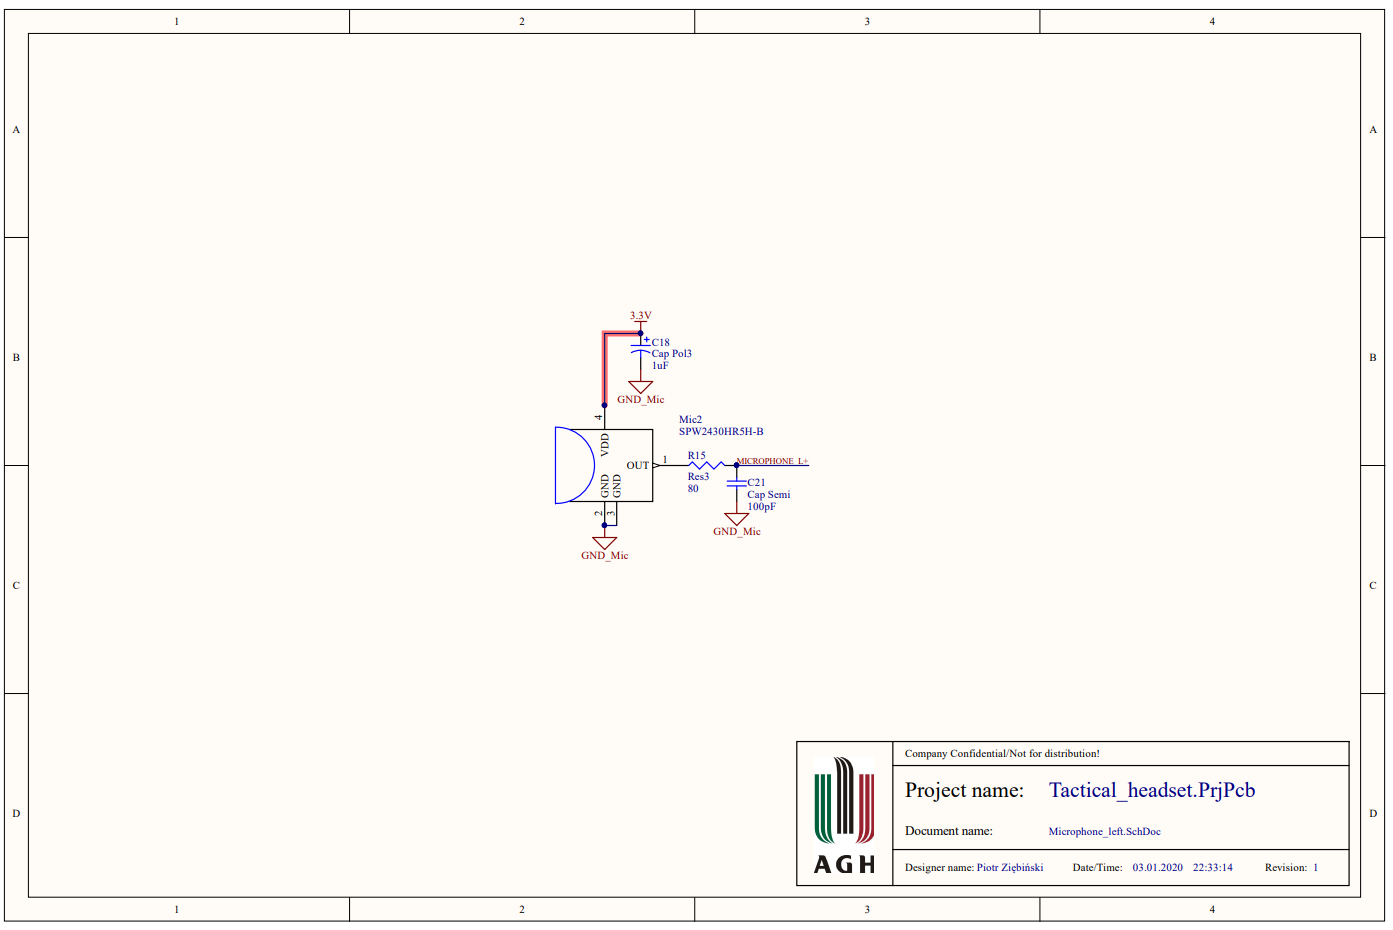
\includegraphics[scale=0.4]{zdjecia/PCB/mic_left.png}
	\caption{\label{mic_left} Schemat \textit{Microphone\_left}}
\end{figure}

\begin{figure}[H]
	\centering
	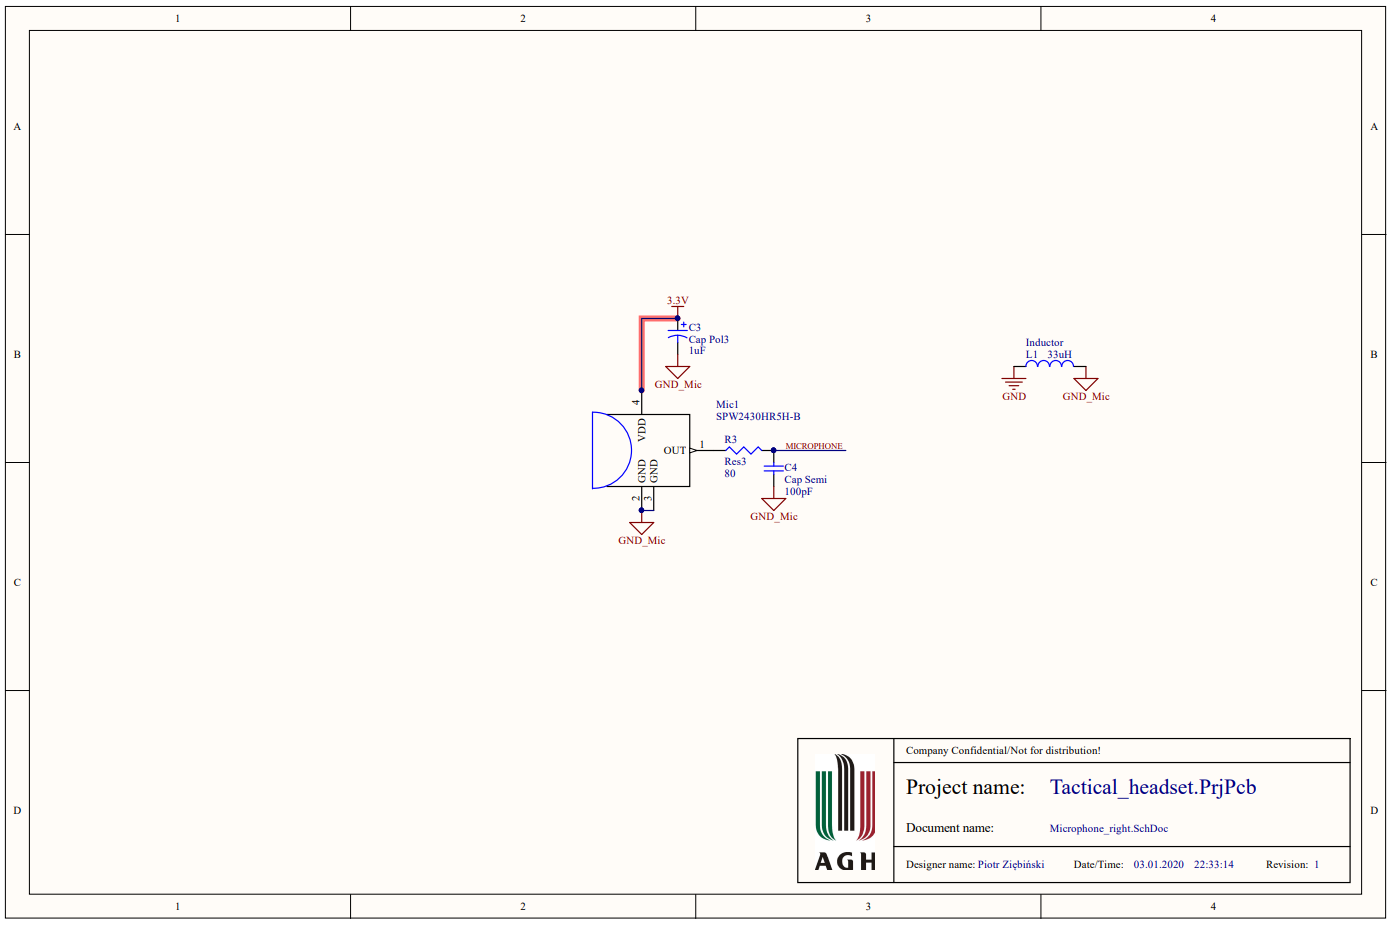
\includegraphics[scale=0.4]{zdjecia/PCB/mic_right.png}
	\caption{\label{mic_right} Schemat \textit{Microphone\_right}}
\end{figure}


\subsection{Speakers}

W przypadku głośników schemat jest wspólny, ponieważ oba wzmacniacze zostały umieszczone na głównym PCB.

Na wyjściach zastosowano filtry LC z częstotliwością graniczną $27khz$ sugerowane w specyfikacji, aby obniżyć szumy EMI. Zasilania również zostały odfiltrowane kondensatorami \textbf{C10} oraz \textbf{C15}.

Na wejściach różnicowych stworzono filtry górnoprzepustowe na $100hz$.

Piny \textbf{SHUTDOWN} zostały podłączone do mikrokontrolera w celu wyłączania wzmacniaczy w trybie uśpienia systemu. Pobierają wtedy maksymalnie $2\mu A$. 

\begin{figure}[H]
	\centering
	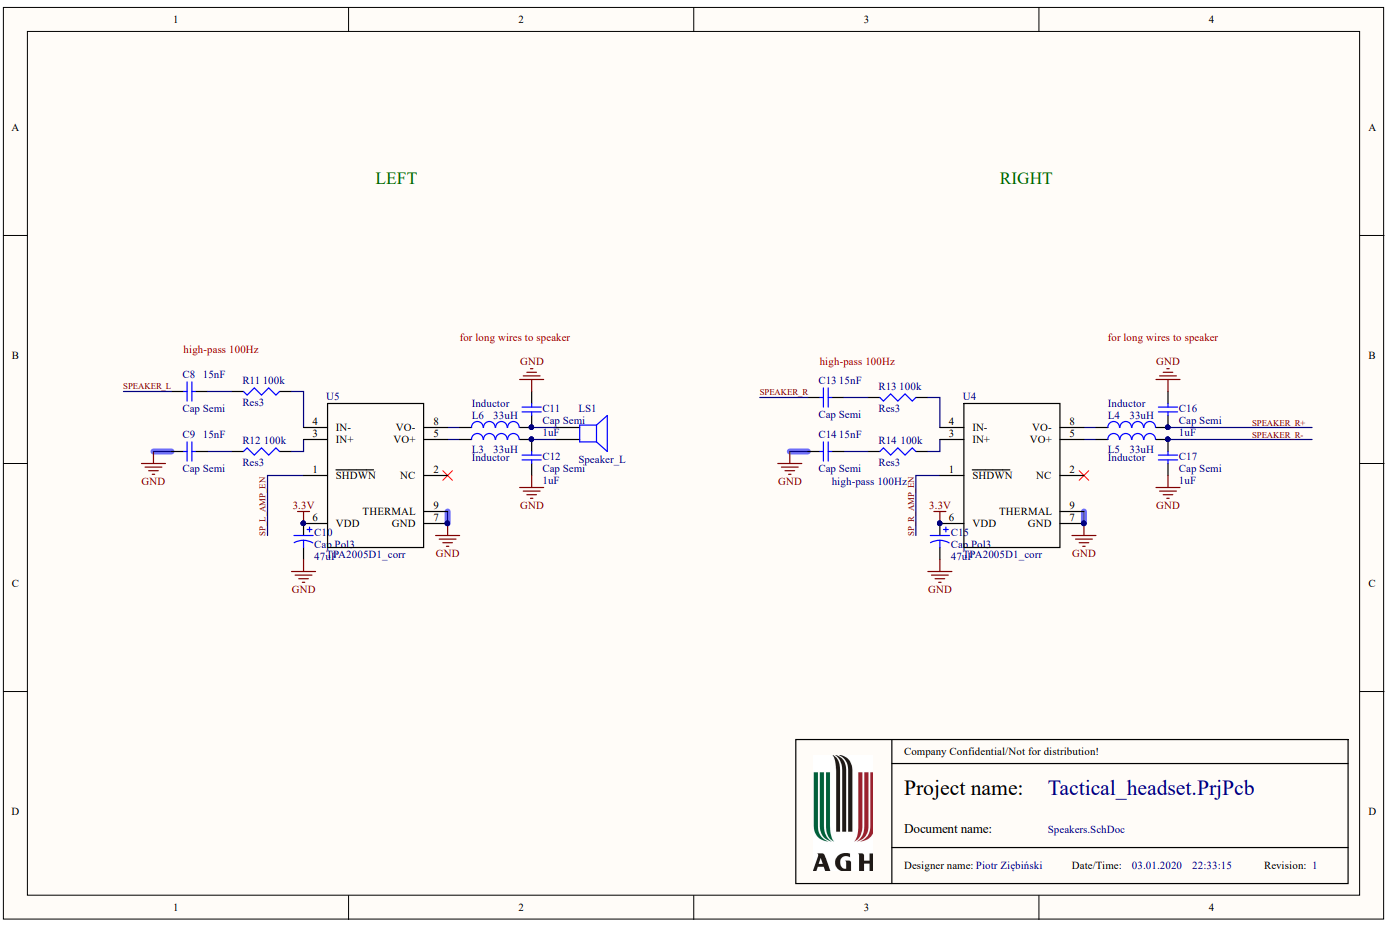
\includegraphics[scale=0.4]{zdjecia/PCB/speakers.png}
	\caption{\label{speakers} Schemat \textit{Speakers}}
\end{figure}


\subsection{Connection}

Schemat stworzony na potrzeby drugiej płytki. Znajdują się na nim: konektor komunikacyjny do głównego PCB, wyjścia do głośnika oraz baterii.

Komunikacja między płytkami odbywa się 6 przewodami: masa, zasilanie $3,3V$, napięcie baterii, dwa sygnały do głośnika i sygnał mikrofonu.

\begin{figure}[H]
	\centering
	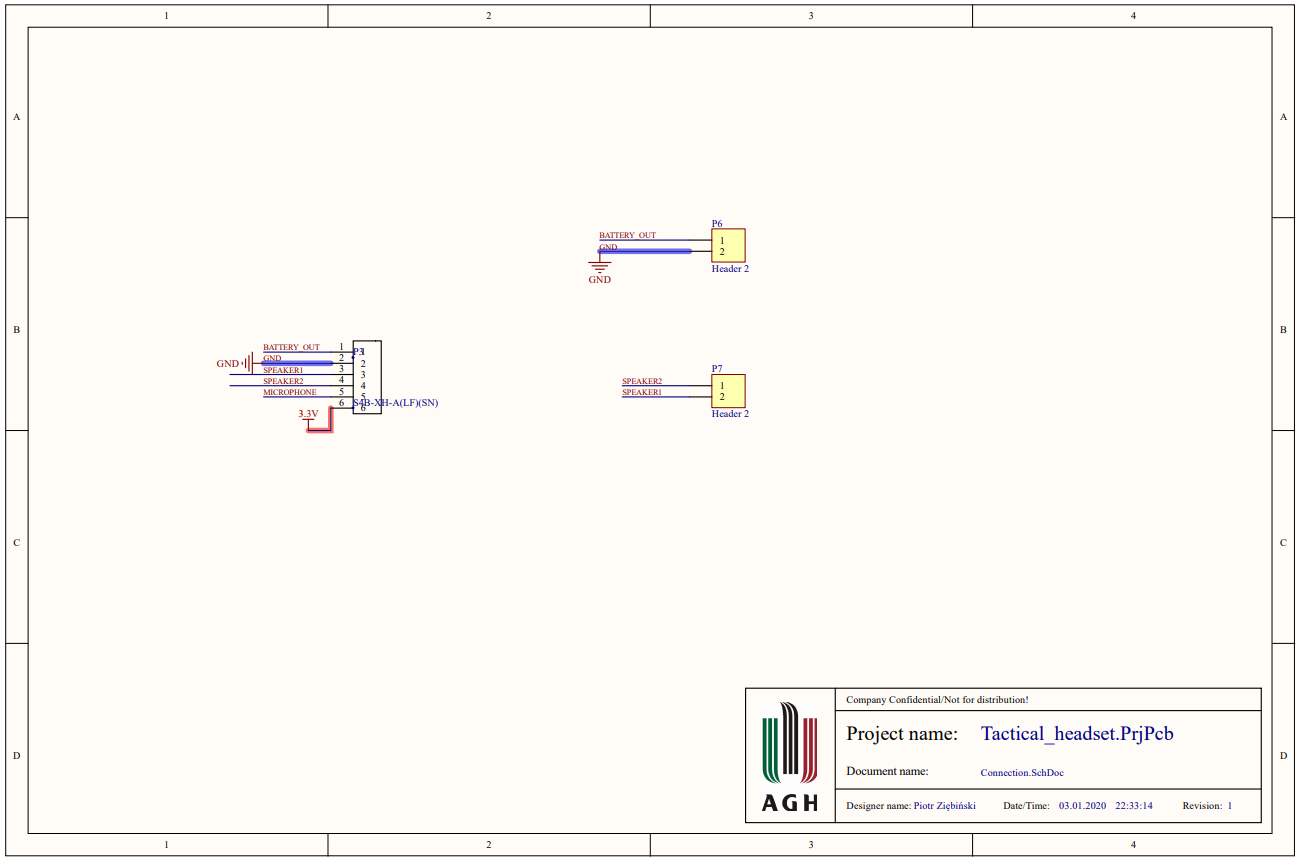
\includegraphics[scale=0.4]{zdjecia/PCB/connection.png}
	\caption{\label{connection} Schemat \textit{Connection}}
\end{figure}


\subsection{PCB\_left}

Jest to główna płytka, na której znajduje się mikrokontroler odpowiedzialny za obliczenia i przetwarzanie sygnałów. Oprócz tego umieszczono na niej przede wszystkim: przyciski, konektor do programowania, do podłączenia radiotelefonu i mikrofonu komunikacyjnego, dwa otwory montażowe wzmacniacze do głośników oraz mikrofon. Ma ona kształt ośmiokąta foremnego o całkowitej szerokości i wysokości $40mm$. Zastosowanie niewielkich wymiarów pozwoliło na łatwe umieszczenie płytki w obudowie i pozostawienie miejsca na materiał wyciszający.

Prawie wszystkie elementy, oprócz mikrofonu i filtrującego jego zasilanie kondensatora, zostały umieszczone na górnej warstwie. Te dwa elementy znajdują się na dole, ponieważ port mikrofonu musiał być skierowany na zewnątrz obudowy i być maksymalnie blisko niej. Do rezystorów zastosowano obudowy 0603, a do kondensatorów i cewek 1206. Utworzone zostały masy \textbf{GND} oraz \textbf{GND\_Mic} na dolnej i górnej warstwie. Związano z nimi także siatkę przelotek łączących obie warstwy ze sobą. Płytka posiada dwa otwory montażowe o średnicach $3,2mm$.

Do mikrofonu komunikacyjnego i połączenia między płytkami zastosowano konektory \textit{JST-XH}. Wyjście głośnika i piny do radiotelefonu przewidziano jako otwory, do których zostaną przylutowane odpowiednie przewody. Natomiast konektor \textbf{SWD} ma służyć jako punkty stykowe do kabla programatora.


\begin{figure}[H]
	\centering
	\begin{subfigure}{.45\textwidth}
		\centering
		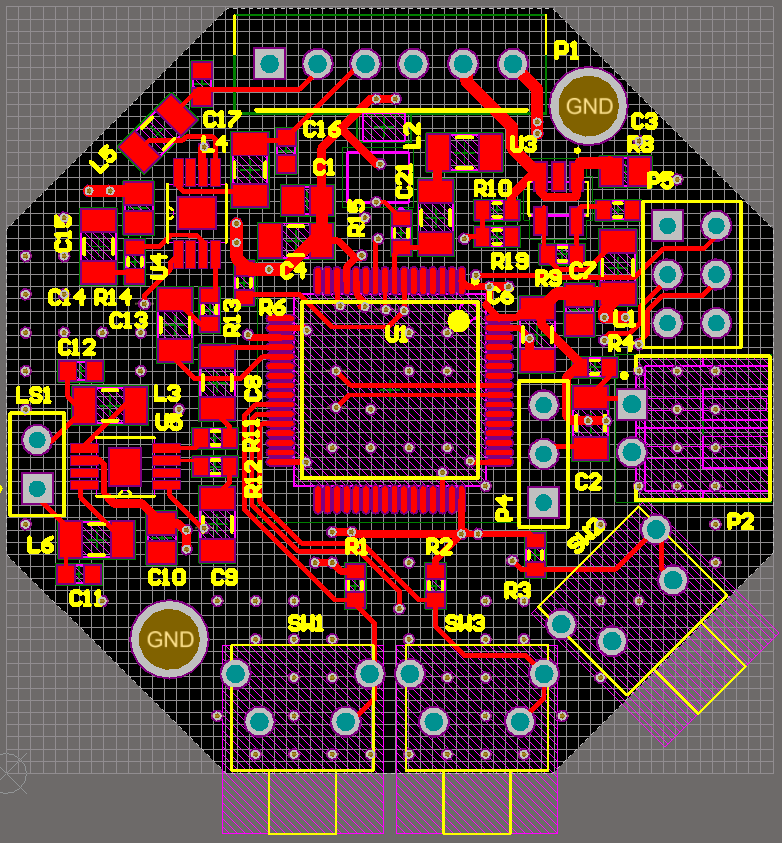
\includegraphics[height=6.5cm]{zdjecia/PCB/PCB_left_top.png}
		\subcaption{Góra}
	\end{subfigure}
	\begin{subfigure}{.45\textwidth}
		\centering
		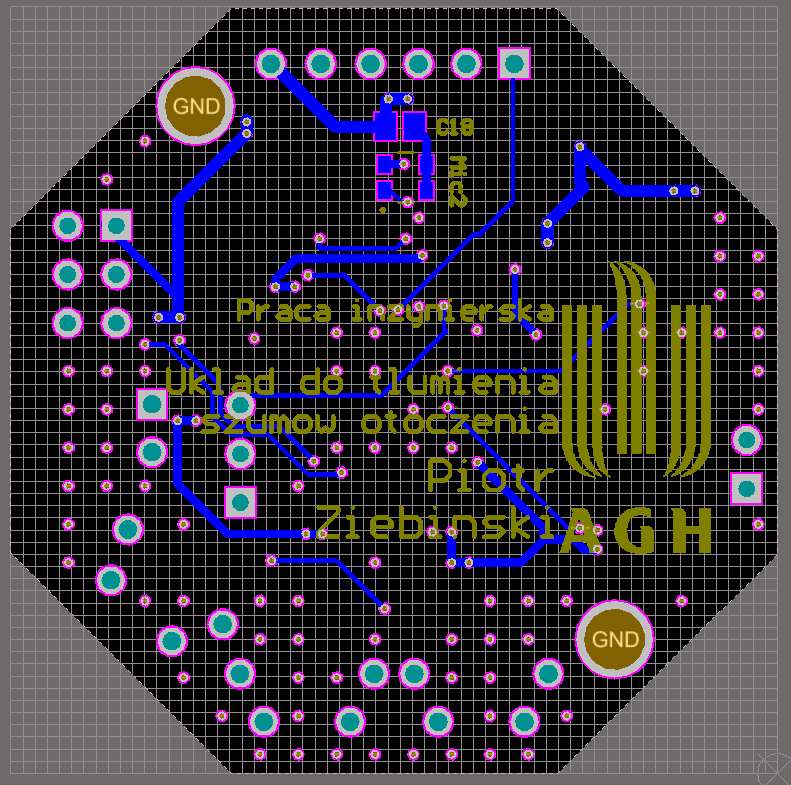
\includegraphics[height=6.5cm]{zdjecia/PCB/PCB_left_bottom.png}
		\subcaption{Dół}
	\end{subfigure}
	\caption{\label{PCB_left} Layout lewej płytki PCB}
\end{figure}

\begin{figure}[H]
	\centering
	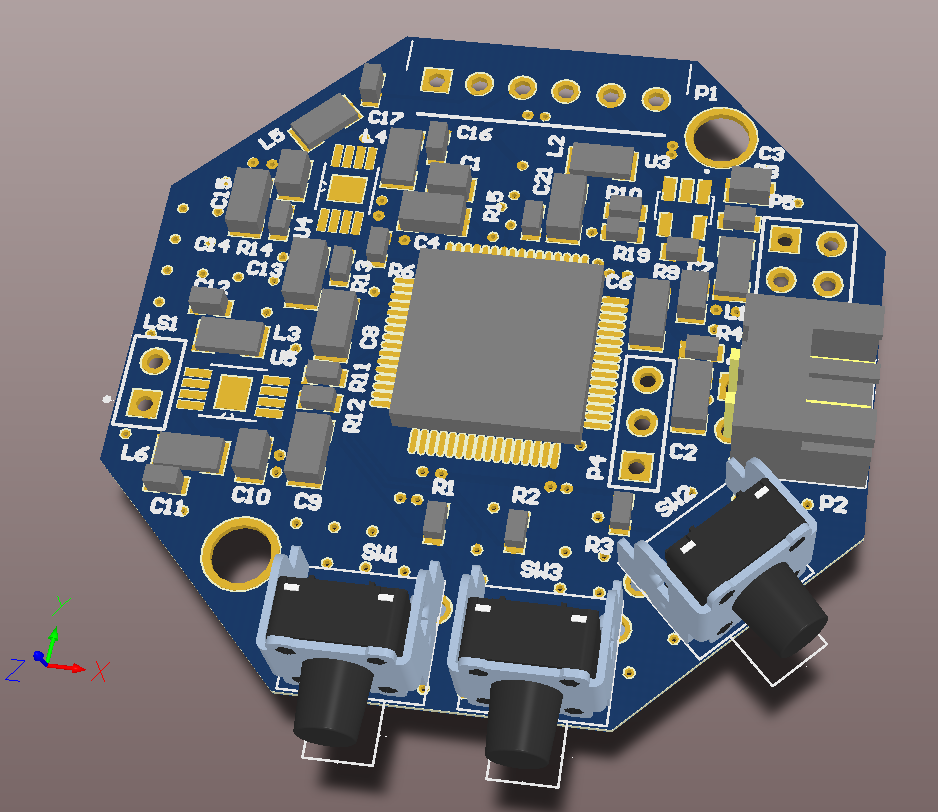
\includegraphics[scale=0.4]{zdjecia/PCB/PCB_left_3D.png}
	\caption{\label{PCB_left_3D} Wygląd płytki z góry w trybie podglądu 3D}
\end{figure}


\subsection{PCB\_right}

Płytka prawa ma znacznie mniejszą funkcjonalność. Z tego powodu jej kształt został ograniczony do prostokąta o wymiarach $15x30mm$. 

Podobnie jak w lewej, tylko mikrofon i kondensator na jego zasilaniu, znajdują się na dolnej warstwie. Płytka zawiera oprócz tego konektor do połączenia do drugiej płytki, wyjścia głośnika i baterii oraz układ ładujący z konektorem mikro USB typu B. Również zastosowano tutaj otwory montażowe oraz po dwie masy na warstwę i dla każdej sieć przelotek.

\begin{figure}[H]
	\centering
	\begin{subfigure}{.45\textwidth}
		\centering
		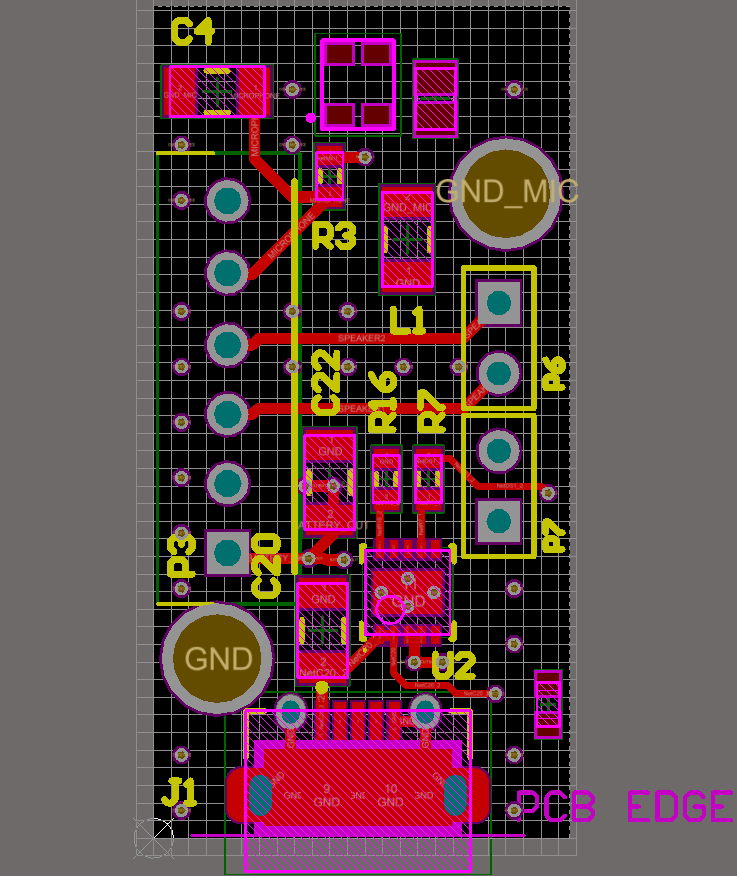
\includegraphics[height=6.5cm]{zdjecia/PCB/PCB_right_top.png}
		\subcaption{Góra}
	\end{subfigure}
	\begin{subfigure}{.45\textwidth}
		\centering
		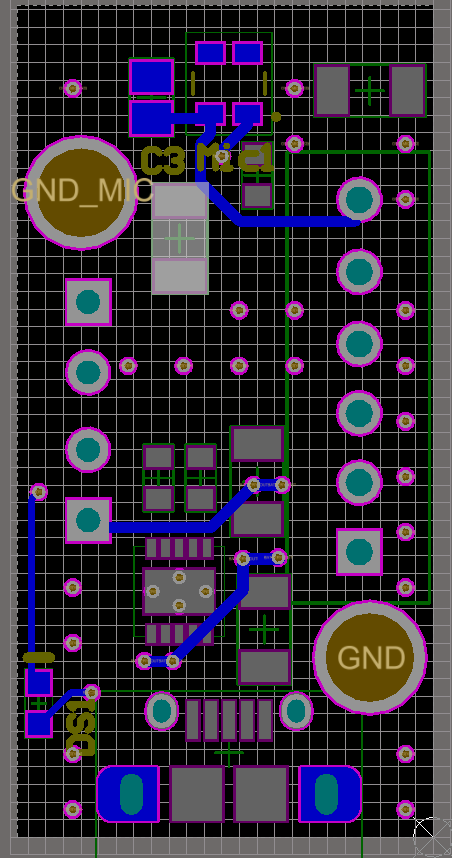
\includegraphics[height=6.5cm]{zdjecia/PCB/PCB_right_bottom.png}
		\subcaption{Dół}
	\end{subfigure}
	\caption{\label{PCB_right} Layout prawej płytki PCB}
\end{figure}

\begin{figure}[H]
	\centering
	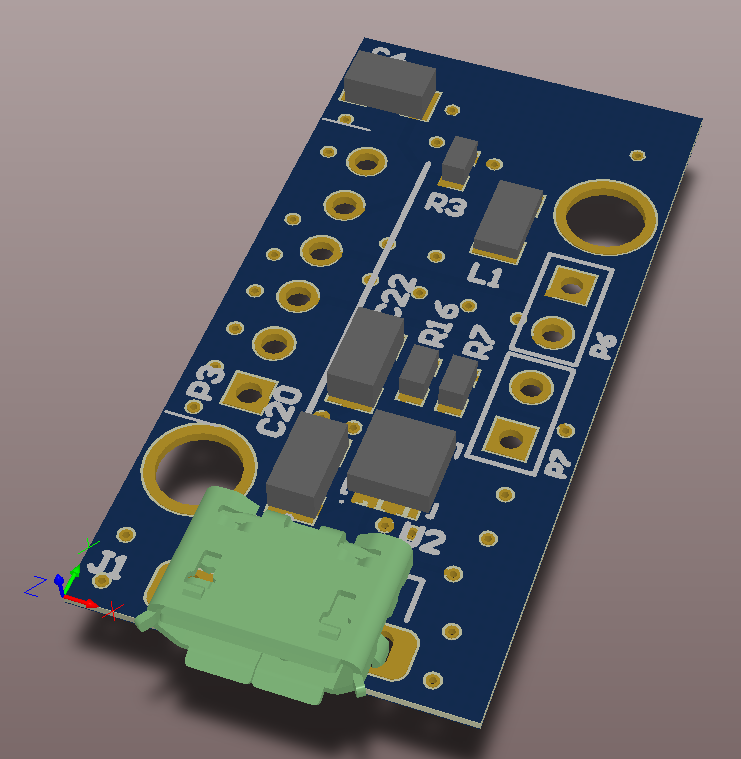
\includegraphics[scale=0.4]{zdjecia/PCB/PCB_right_3D.png}
	\caption{\label{PCB_right_3D} Wygląd prawej płytki z góry w trybie podglądu 3D}
\end{figure}

\section{Pobór mocy}
\label{cha:pobor_mocy}

\textbf{NIE WIEM JAK TO POLICZE, ALE CHYBA JAKOŚ POWINIENEM}


